\documentclass[tikz,border=8pt]{standalone}
\usepackage{amsmath}
\usepackage{pgfplots}
\pgfplotsset{compat=1.18}

\definecolor{ink}{HTML}{21352F}
\definecolor{teal}{HTML}{087F7B}
\definecolor{blue}{HTML}{4B77A8}
\definecolor{gold}{HTML}{C58B2A}
\definecolor{rose}{HTML}{B65A62}

\begin{document}
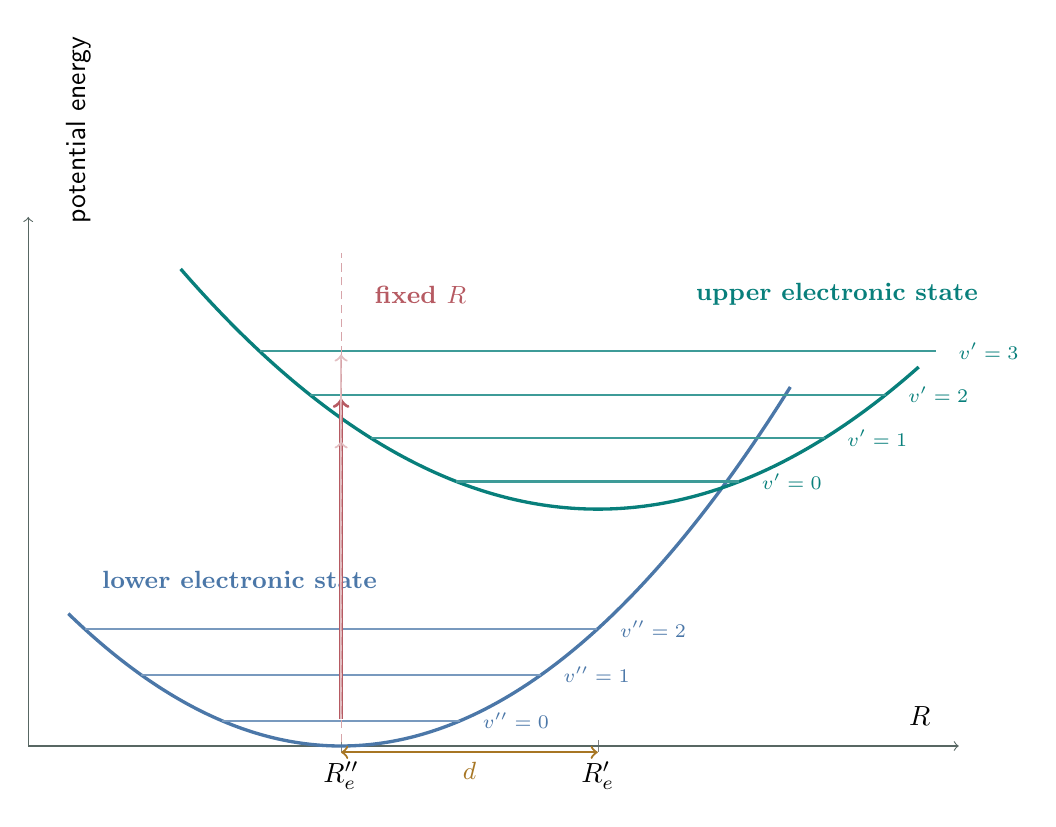
\begin{tikzpicture}[font=\sffamily]
\begin{axis}[
  width=13.4cm,
  height=8.3cm,
  xmin=.45,xmax=6.25,
  ymin=0,ymax=6.7,
  axis lines=left,
  axis line style={draw=ink!75,->},
  xlabel={$R$},
  ylabel={potential energy},
  xtick={2.4,4.0},
  xticklabels={$R_e''$,$R_e'$},
  ytick=\empty,
  xlabel style={at={(axis description cs:.98,.02)},anchor=south east},
  ylabel style={at={(axis description cs:.03,.97)},anchor=north west},
  clip=false
]
  \addplot[blue,very thick,domain=.7:5.2,samples=160]
    {.58*(x-2.4)^2};
  \addplot[teal,very thick,domain=1.4:6.0,samples=160]
    {3.0+.45*(x-4.0)^2};

  \node[blue,font=\small\bfseries,anchor=west]
    at (axis cs:.85,2.1) {lower electronic state};
  \node[teal,font=\small\bfseries,anchor=west]
    at (axis cs:4.55,5.72) {upper electronic state};

  % Lower-state levels from exact intersections with U''=.58(R-2.4)^2.
  \foreach \lev/\lab in {.32/0,.90/1,1.48/2}{
    \pgfmathsetmacro{\dx}{sqrt(\lev/.58)}
    \pgfmathsetmacro{\xl}{2.4-\dx}
    \pgfmathsetmacro{\xr}{2.4+\dx}
    \pgfmathsetmacro{\xn}{2.48+\dx}
    \edef\levelcommand{
      \noexpand\draw[blue!75,thick]
        (axis cs:\xl,\lev)--(axis cs:\xr,\lev);
      \noexpand\node[blue,font=\noexpand\scriptsize,anchor=west]
        at (axis cs:\xn,\lev) {$v''=\lab$};
    }
    \levelcommand
  }

  % Upper-state levels from exact intersections with U'=3+.45(R-4)^2.
  \foreach \lev/\lab in {3.35/0,3.90/1,4.45/2,5.00/3}{
    \pgfmathsetmacro{\dx}{sqrt((\lev-3.0)/.45)}
    \pgfmathsetmacro{\xl}{4.0-\dx}
    \pgfmathsetmacro{\xr}{4.0+\dx}
    \pgfmathsetmacro{\xn}{4.08+\dx}
    \edef\levelcommand{
      \noexpand\draw[teal!78,thick]
        (axis cs:\xl,\lev)--(axis cs:\xr,\lev);
      \noexpand\node[teal,font=\noexpand\scriptsize,anchor=west]
        at (axis cs:\xn,\lev) {$v'=\lab$};
    }
    \levelcommand
  }

  % All arrows have exactly the same x coordinate: fixed R.
  \draw[rose,very thick,->]
    (axis cs:2.4,.34)--(axis cs:2.4,4.40);
  \draw[rose!38,thick,->]
    (axis cs:2.4,.34)--(axis cs:2.4,3.86);
  \draw[rose!38,thick,->]
    (axis cs:2.4,.34)--(axis cs:2.4,4.96);
  \draw[rose!55,densely dashed]
    (axis cs:2.4,.05)--(axis cs:2.4,6.25);
  \node[rose,font=\small\bfseries,anchor=west]
    at (axis cs:2.55,5.72) {fixed $R$};

  \draw[<->,gold!85!black,thick]
    (axis cs:2.4,-.08)--(axis cs:4.0,-.08)
    node[midway,below,font=\small] {$d$};
\end{axis}
\end{tikzpicture}
\end{document}
